\chapter{子痫前期及脉搏波的生理学基础}
\section{引言}
子痫前期会引起孕妇机体一系列复杂的生理、病理反应,会对孕妇患者全身各脏器、各系统等造成不良影响。本章详细阐述子痫前期引起的生理变化及危害,介绍脉搏波的产生机理、采集原理、常见的生理参数与非生理参数模型等方面,
并从方法论的角度概括脉搏波分析研究的本质。

本章研究内容的框架图如\autoref{fig:frameworks2}所示。
\begin{figure}[htbp]
    \centering
    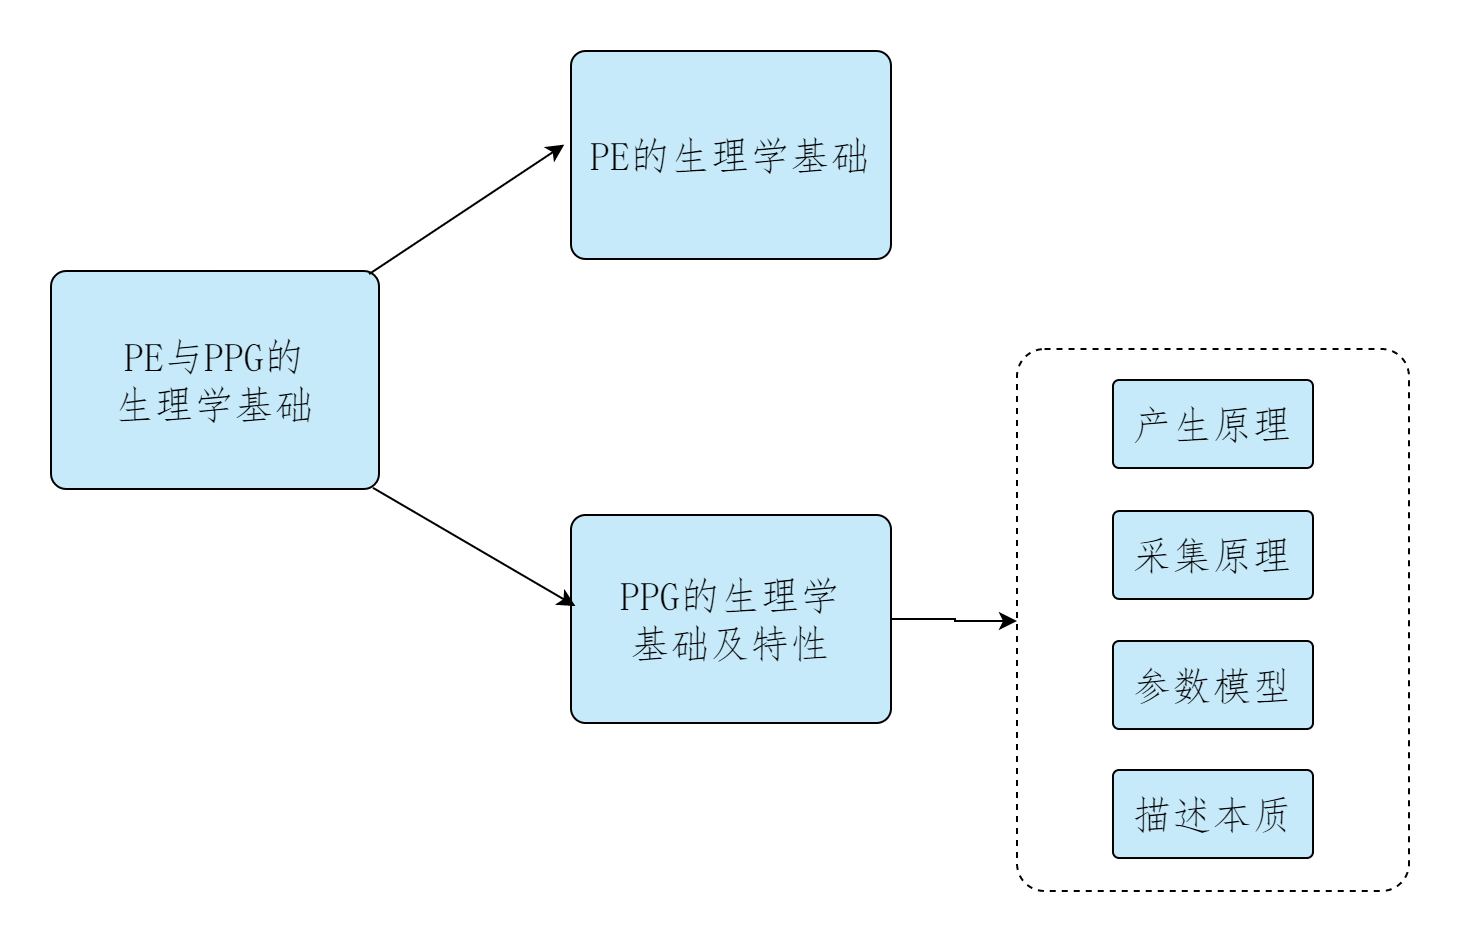
\includegraphics[width=.75\linewidth]{pe/frameworks2} 
    \caption{\label{fig:frameworks2}第二章研究内容框架图}
\end{figure}

\section{子痫前期的生理学基础}
PE引起的基本的病理生理变化包括全身小动脉痉挛、血管内皮损伤和水钠潴留等\cite{OAG9}。可能由于升压系统和降压系统平衡失调,血管壁对血管紧张素Ⅱ等升压物质的反应性增强,从而使全身小动脉
(特别是直径200$um$以下的小动脉)发生痉挛,导致各器官供血不足,外周阻力增高,产生高血压等一系列症状。全身各脏器各系统灌注减少,对母婴造成危害,甚至导致母婴死亡。由于PE表现为多脏器和系统损害,
故有学者提出子痫前期-子痫综合征(preeclampsia-eclampsia syndrome,PES)的概念\cite{OAG9}。

孕妇PE病发后,其全身各器官组织的正常功能均会受到一定的影响,可能出现的病生理变化包括以下方面\cite{OAG9}:

一、脑

脑部血管痉挛,通透性增加,导致脑组织缺氧并进一步产生水肿、充血、局部缺血、血栓形成及出血等现象。CT检查脑皮质呈现低密度区,并有相应的局部缺血和点状出血,提示脑梗死。
此时孕妇可能会出现头昏、头痛、恶心、呕吐等症状,个别严重者会抽搐、昏迷,甚至形成脑疝而致死亡。

二、肾脏

肾脏血管痉挛引发肾小球扩张,内皮细胞肿胀,纤维素沉积于内皮细胞。血浆蛋白从肾小球漏出导致孕妇出现蛋白尿。肾血流量下降引起组织缺氧,使肾小球滤过量下降,导致血尿酸和肌酐水平升高。孕妇出现尿少等症状,严重者可致肾功衰竭。
此外,可能由于肾小球滤过率减少,肾小管对钠的重吸收增加,钠离子潴留细胞外而引起水肿,导致孕妇体重异常增加。

三、肝脏

肝脏由于缺血,肝细胞线粒体内所含的谷丙转氨酶释放,可致血清谷丙转氨酶升高,出现黄疸。肝脏出现特征性损伤,门静脉周围有局限性出血,继而纤维素性血栓形成,严重时门静脉周围坏死和肝包膜下血肿形成,甚至发生肝破裂危及母婴生命。

四、心血管

心脏血管痉挛,血压升高,同时由于血液粘稠度增加,外周阻力增加,心肌收缩力受损和射血阻力(即心脏后负荷)增加,心输出量明显减少。此时心血管系统处于低排高阻状态,而内皮细胞活化使血管通透性增加,血管内
液进入心肌细胞间质,导致心肌缺血、间质水肿、心肌点状出血或坏死,严重时导致心力衰竭,继而发生肺水肿。

五、血液

由于全身小动脉痉挛,血管壁渗透性增加,血液浓缩,血细胞比容上升。当血细胞比容下降时,多合并贫血或红细胞受损或溶血。

六、内分泌及代谢

由于血管紧张素转化酶增加,妊娠晚期盐皮质激素、去氧皮质酮升高可致钠潴留,血浆胶体渗透压降低,细胞外液可超过正常妊娠,但水肿与子痫前期的严重程度及预后关系不大。
通常其电解质水平与正常妊娠无明显差异。子痫抽搐后,可出现乳酸性酸中毒及呼吸代偿性的二氧化碳丢失,可致血中碳酸盐浓度降低。

七、子宫胎盘血流灌注

子宫血管痉挛,子宫螺旋动脉重铸不足导致胎盘灌注下降,螺旋动脉平均直径仅为正常孕妇螺旋动脉直径的一半。常伴有内皮损害及胎盘血管急性动脉粥样硬化,使胎盘供血不足,绒毛退行性变、出血、坏死、梗塞等,
导致胎盘提高老化,功能不全。病变进行缓慢时,可致胎儿宫内生长发育迟缓;病变急剧时,可致胎死宫内,严重时胎盘后小血管破裂,导致胎盘早剥。

\section{脉搏波的生理学基础及特性}
本节将从脉搏波的产生原理、采集原理、典型特征及参数描述的本质等四方面对脉搏波进行介绍。

\subsection{脉搏波产生原理}
与心电产生原理类似,脉搏波也是由心脏周期性收缩与舒张引发的节律间歇性射血所产生的,其波形与心电有一定的关联性,如\autoref{fig:ecgppg}所示\cite{Allen2007}。
脉搏波蕴含着丰富的血液动力学信息,可以通过其形态、强度、速率、节律等特征反映心脏的功能与状态,也可以反映出各级动脉及分支中血管壁弹性、血管阻力、血液黏度等信息。
由于血管系统本身的阻力与弹性,射血引起的主动脉扩张与收缩最终导致血液
以压力波动的形式从主动脉传播、延伸至整个血管动脉系统。脉搏波在颈动脉、肱动脉、桡动脉等浅表动脉可以直接通过手指在皮肤表面感受到\cite{PPGYY}。
\begin{figure}[htbp]
    \centering
    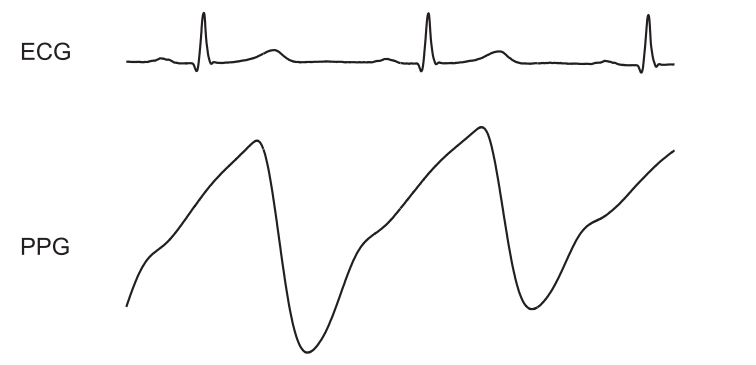
\includegraphics[width=.6\linewidth]{pe/ecgppg}
    \caption[心电与脉搏波信号示意图]{\label{fig:ecgppg}心电与脉搏波信号示意图\cite{Allen2007}}
\end{figure}

脉搏波在血管动脉系统中传播时,脉搏压力波的部分能量会从不同位置反射回心脏。由于不同动脉段管壁弹性存在差异、动脉在某些部位出现分叉管以及血管本身狭窄等因素,动脉管系中会出现一系列特殊的间断点。
间断点两侧出现的阻抗突变会导致脉搏波在间断点上发生不同程度的折射和反射。动脉中向心的反射波在到达动脉瓣处后,会发生二次反射,这会导致脉搏波中重搏波的出现。
这时,整个动脉管系的脉搏波传播过程可以视为这些间断点处各个行波线性叠加的结果\cite{THOCBPM}。不同间断点处的反射特征不尽相同,其中小动脉、微动脉与毛细血管由于具有更大的阻抗,是脉搏波反射的最主要部位,如\autoref{fig:artery}所示。
其中,左心室输出的原发脉搏波在肾动脉与髂分叉动脉附近产生了两个反射波,这两个反射波在\autoref{fig:artery}中分别用深黑色与浅蓝色进行了区分标注。
\begin{figure}[htbp]
    \centering
    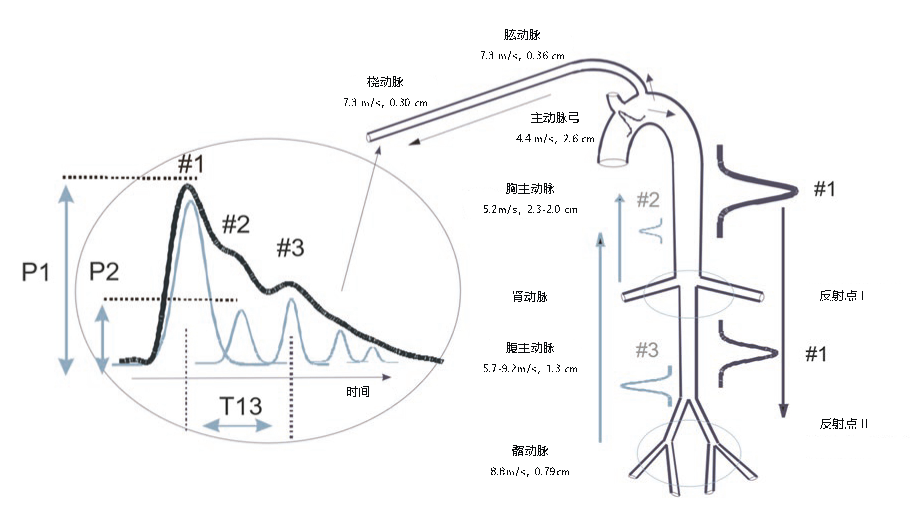
\includegraphics[width=0.9\linewidth]{pe/artery}
    \caption[主动脉-手臂复合动脉系统及其对桡动脉-指动脉处动脉脉搏波的影响示意图]{\label{fig:artery}主动脉-手臂复合动脉系统及其对桡动脉-指动脉处动脉脉搏波的影响示意图\cite{THOCBPM}}
\end{figure}

\subsection{光电容积脉搏波采集原理}
根据检测方式的不同,可将脉搏波分为压力脉搏波和容积脉搏波两类。压力脉搏波主要表征血管内血液压力的传输,容积脉搏波主要表征外周血管与微循环中等微血管血液容积的脉动性变化。
其中,光电容积脉搏波(photoplethysmography,PPG)最早于1937年由Hertzman等\cite{Hertzman1937}提出,是利用光电转换方法检测组织中血液容积变化的一种技术。

PPG的检测可依据光的接收方式分为透射式与反射式两种\cite{THOCBPM},透射式PPG采集时,光源与传感器对称分布,其原理是使用一定波长光源照射在人体组织表面,由于皮肤、血液、肌肉等各组织的吸收作用,一部分光发生漫反射,
一部分光透过组织被传感器接收。反射式PPG采集原理与透射式基本相同,区别在于反射式下传感器被放置在光源同侧以接收漫反射回来的光\cite{THOCBPM,mmt},如\autoref{fig:led}所示。
透射式PPG检测一般多用于人体耳垂、指端等部位,反射式PPG一般多用于手腕、
胸部等其他表层血管发达区域\cite{THOCBPM}。一般认为,透射式检测更方便指示心率的时间关系,而反射式则对于血管容积变化的检测更有优势\cite{mmt}。
\begin{figure}[htbp]
    \centering
    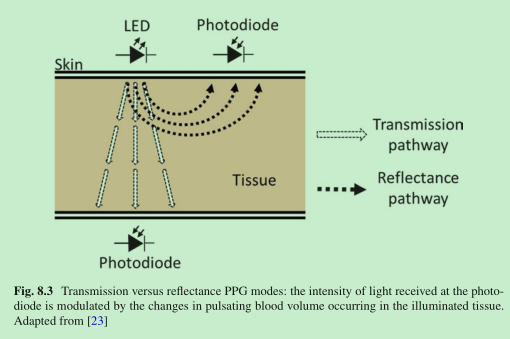
\includegraphics[width=.7\linewidth]{pe/led}
    \caption[PPG检测的两种方式示意图]{\label{fig:led}PPG检测的两种方式示意图\cite{THOCBPM}}
\end{figure}

当心脏收缩时,外周血容量最多,光吸收量也最大,故检测到的光强度最小;而在心脏舒张时则恰恰相反,外周血容最小,光的吸收量最小,检测到的光强度最大\cite{lhc,cwl}。
在物理光学中,将光通过某种透明介质后被吸收的比例定义为光的吸收度$A$
\begin{equation}
    \label{equ:LBL}
    A=\lg\frac{I_{0}}{I_{T}}
\end{equation}

其中,$I_{0}$与$I_{T}$分别是入射光强度与透射光强度。而朗伯-比尔定律(Lambert-Beer's law)指出,光的吸收度与入射光的强度无关,在光程上每等厚层介质吸收相同比例值的光,即:
\begin{equation}
    \label{equ:LBL2}
    A=C \cdot \varepsilon \cdot V
\end{equation}
其中,$V$是透明介质的体积,$C$是透明介质的浓度,$\varepsilon$则是吸收系数,$\varepsilon$一般与透明介质的性质、入射光波长及温度等因素相关。

在透射式的PPG检测中,考虑到人体指端各组织对入射光的均有吸收,若忽略由于散射、反射等因素造成的衰减,以波长为$\lambda$的单色光垂直照射指端,则最终指端透射光强度为\cite{4122392}:
\begin{equation}
    \label{equ:AF1}
    I=I_{0}e^{-C_{t}\varepsilon _{t}V_{t}}e^{-C_{v}\varepsilon _{v}V_{v}} e^{-C_{a}\varepsilon _{a}V_{a}} 
\end{equation}

\begin{figure}[htbp]
    \centering
    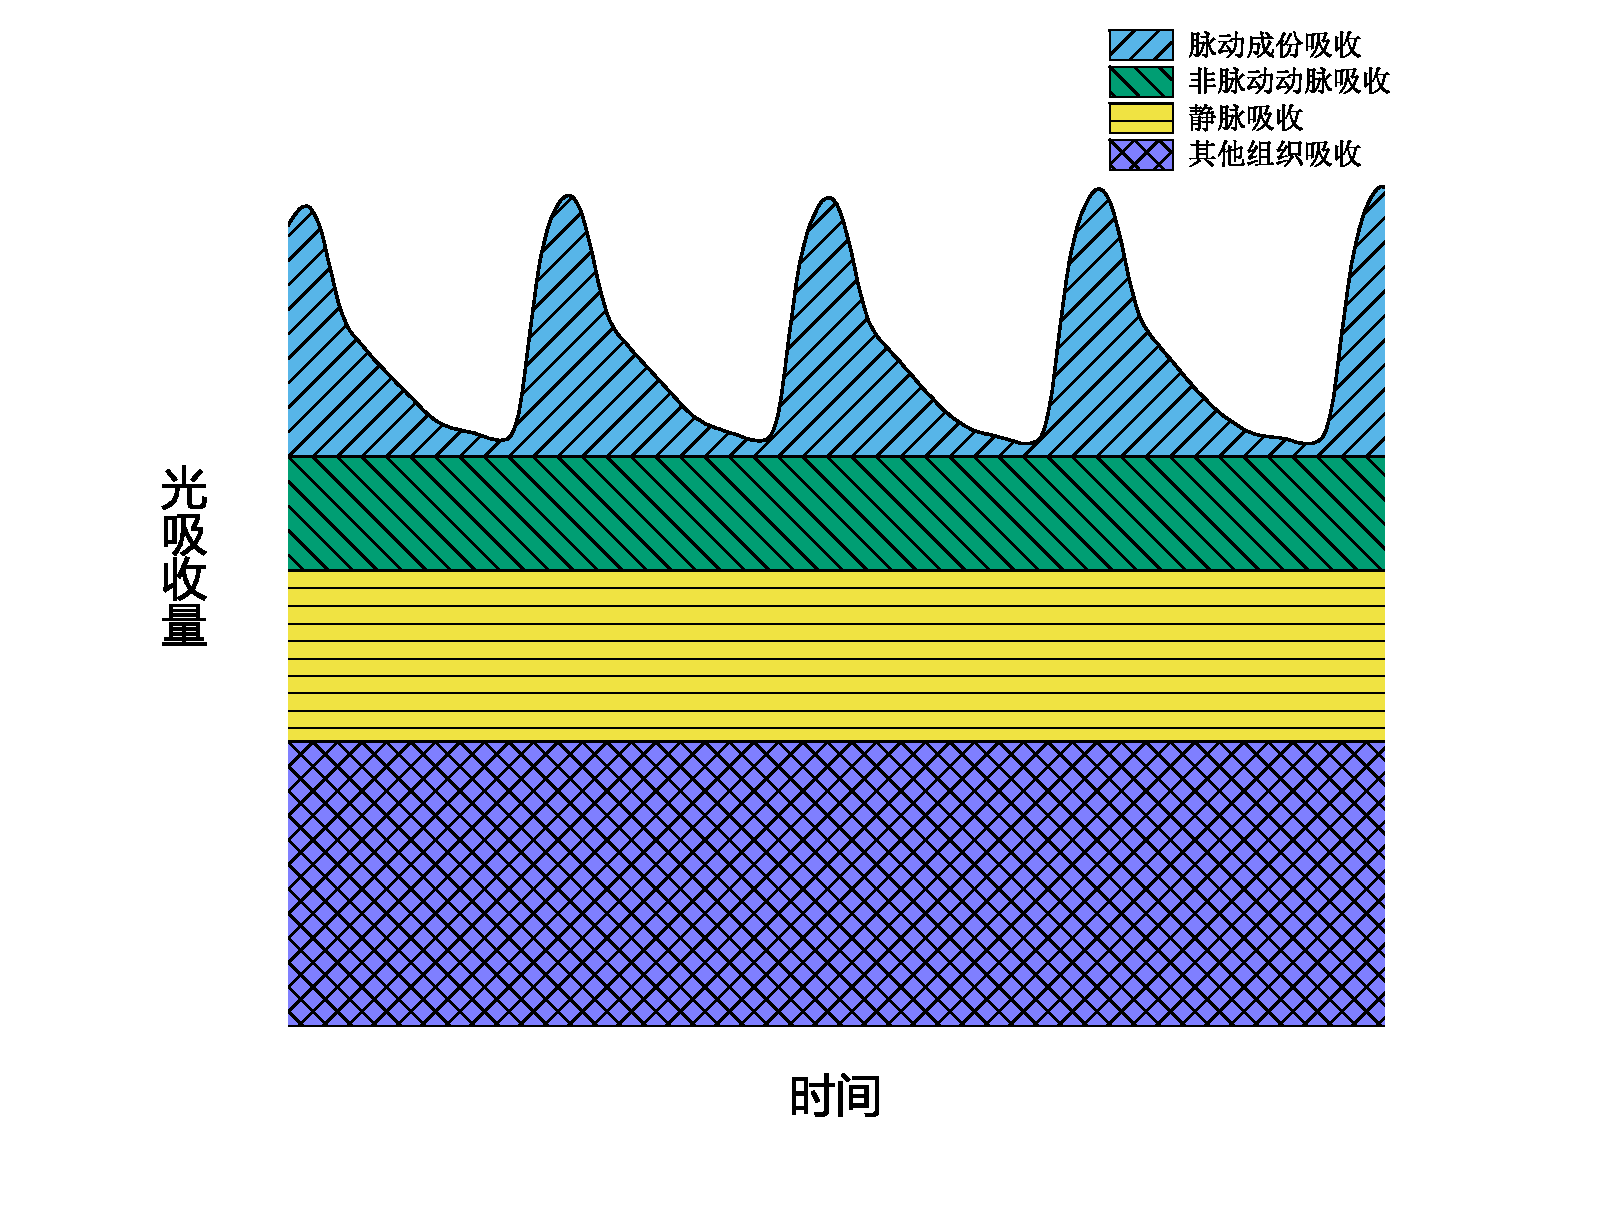
\includegraphics[width=.6\linewidth]{pe/absorb}
    \caption{\label{fig:absorb}PPG的光吸收示意图}
\end{figure}

其中,下标$t$、$v$、$a$分别代表皮肤肌肉组织、静脉血液、动脉血液等成分。学者们已经证实皮肤肌肉组织、静脉血液等组织对光的吸收是恒定不变的\cite{1980Spectrophotometric,4122392},如\autoref{fig:absorb}所示。
因此,可对\autoref{equ:AF1}进行精简,以表示通过动脉血液的透光强度\cite{PPGYY}:
\begin{equation}
    \label{equ:AF2}
    I=I_{0}e^{-C_{a}\varepsilon _{a}V_{a}} 
\end{equation}

当动脉血液的容积因心脏搏动而发生极小的变化$\Delta V_{a}$时,透光强度也将随之变动,将其记为$\Delta I$,则\autoref{equ:AF2}可改写为:
\begin{equation}
    \label{equ:AF3}
    I+\Delta I=I_{0}e^{-C_{a}\varepsilon _{a}(V_{a}+\Delta V_{a})} 
\end{equation}

将\autoref{equ:AF2}与\autoref{equ:AF3}相除,可得:
\begin{equation}
    \label{equ:AF4}
    \frac{I+\Delta I}{I}=\frac{I_{0}e^{-C_{a}\varepsilon _{a}(V_{a}+\Delta V_{a})}}{I_{0}e^{-C_{a}\varepsilon _{a}V_{a}}}=e^{-C_{a}\varepsilon _{a}\Delta V_{a}} 
\end{equation}

进一步,对\autoref{equ:AF4}两边同时取对数,并根据数学近似关系
\begin{equation}
    \label{equ:lnx}
    \ln(1+x)\approx x,x\rightarrow 0
\end{equation}
可得:
\begin{equation}
    \label{equ:AF5}
    \frac{\Delta I}{I}=-C_{a}\varepsilon _{a}\Delta V_{a}
\end{equation}

将\autoref{equ:AF2}代入\autoref{equ:AF5},稍作整理可得:
\begin{equation}
    \label{equ:AF6}
    \frac{\Delta V_{a}}{V_{a}}=\frac{1}{\ln(I/I_{0})}\frac{\Delta I}{I}
\end{equation}

由\autoref{equ:AF6}可知,与个体相关性强的动脉血总的光吸收系数$\varepsilon _{a}$、动脉血浓度$C_{a}$等变量最终均与指端血液容积变化率$\Delta V_{a}/{V_{a}}$无关。
若在一个完整的测量周期内保持入射光强度$I_{0}$不变,即可消除上式中$I_{0}$对结果的影响。此时指端血液容积变化率$\Delta V_{a}/{V_{a}}$与容积透射的光强变化率$\Delta I/I$成正比例关系,从而排除了个体差异等因素的影响
\cite{1980Spectrophotometric,4122392,PPGYY}。PPG信号检测正是依此原理,通过光电转换硬件电路检测光信号并从光强变化率中获取指端血液容积变化率的信息。

\subsection{光电容积脉搏波的典型特征}
作为人体电生理内源信号的一种,PPG不仅拥有一般医学信号的共性特征,还拥有其鲜明的个性特点。

一、共性特征

PPG信号是一种平稳随机信号,和其他人体内源信号类似,有着医学信号的以下特点\cite{Ma2015,Qiu2012,Naraharisetti2011,Miao2020,LMX2019}。

1、信号弱

PPG信号源于心脏搏动,在体表检测到的信号幅值低,一般都在$mV$级别,属于微弱电信号。

2、频率低

PPG以低频信号为主,频谱范围是0.1$\sim$40Hz,其信号能量主要集中在5Hz以内。其中,心脏搏动信号能量集中在0.5$\sim$4Hz,呼吸引入的能量集中在0.2$\sim$0.35Hz。

3、易受干扰

由于PPG信号弱、频率低,在检测时极易受到各种噪声干扰。工频干扰是最常见的噪声信号源,采集过程中被试发生体动也很容易干扰检测结果。此外,由于PPG信号光电采集的特殊性,环境光亮度等因素也会影响最终的结果。

4、随机性强

由于人体系统的时变性、复杂性及个体差异性,使得PPG信号具有显著的随机性,即使同一个人在不同时间段的脉搏波也不一定相同。

二、个性形态特征

一个完整的PPG波形包括上升支和下降支两部分。在心脏的快速射血期,心脏收缩,血液开始进入主动脉,血管壁扩张,动脉血压快速上升,形成脉搏波的上升支。
这个过程非常迅速,因此上升支大多较为陡峭。快速射血期结束时,动脉压力达到最大,PPG也达到波峰,上升支结束。此后进入心室射血后期,射血速度减慢,
进入主动脉的血液容量小于从主动脉流入外周血管的血液容量,动脉开始回缩,主动脉压力减小,形成降支前段。随后心脏射血期结束,心室开始舒张,动脉血压继续下降,
直到开始下一个心动周期。下降支中可能还会出现潮波和重搏波,其波形特征与血管张力、管道阻力和血管弹性有关\cite{PPGYY,Chen2021}。

典型的PPG波形如\autoref{fig:ppg}所示,其中A为主波波峰,
B为潮波(重搏前波),C为重搏波波谷,D为重搏波波峰,E为主波波谷。
\begin{figure}[htbp]
    \centering
    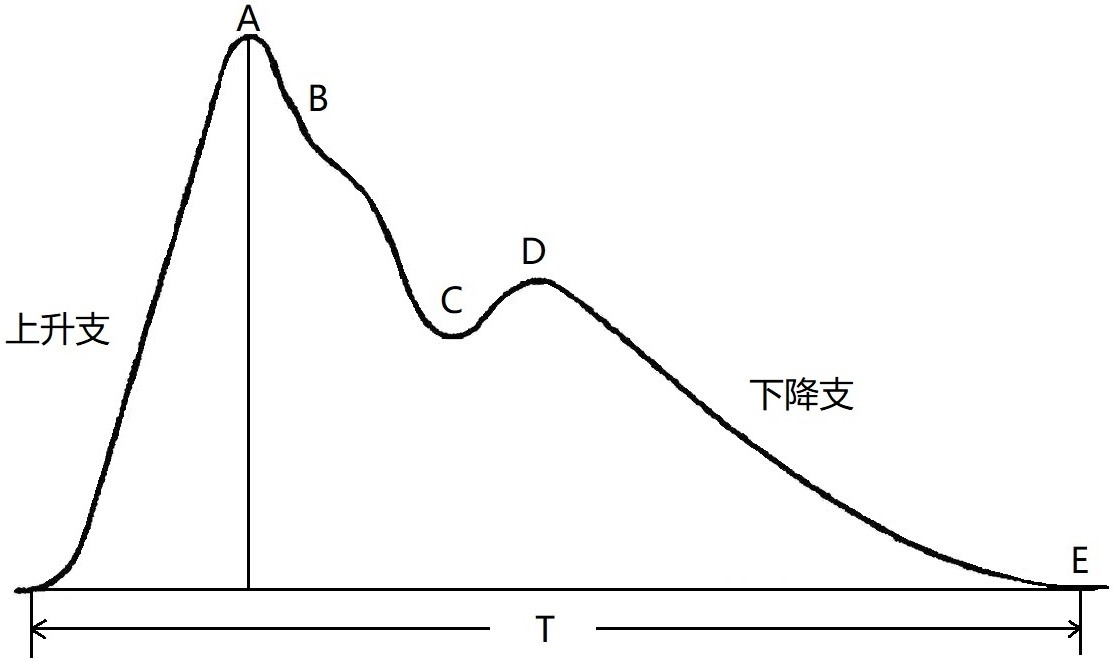
\includegraphics[width=.6\linewidth]{pe/ppg} 
    \caption{\label{fig:ppg}PPG波形示意图}
\end{figure}

\subsection{生理参数与非生理参数建立的微循环模型}
按照信号与系统的观点,若干相互作用、相互联系的事物按一定规律组成具有特定功能的整体均可称为系统,而信号则是反映信息的各种物理量,是系统直接进行加工、变换以实现通信的对象\cite{Alan2019}。而在脉搏波的工程研究领域,
人体的动脉管系亦可视为一个力学系统,心脏搏动作为该系统输入,而人体各处采集获得的脉搏波即为该系统输出(响应)。可由该系统的输入输出关系分析推断其结构特性参数,进一步研究脉搏波其他特性\cite{PPGYY}。

临床上一般将动脉系统末梢的微动脉和微静脉之间的血液循环称为微循环\cite{Abraham2011,John2004}。
为尽可能精确描述心血管系统、探求心血管系统的生理特性,多年来学者们提出并建立了各种不同的数学模型对其进行拟合。依据模型建立时是否使用多个变量去拟合还原血液在血管中的可能涉及的血压、
血流弹性、阻力等生理变量,这些心血管模型大体上可分为生理参数模型与非生理参数模型两大类。

一、生理参数模型

生理参数模型关注心血管系统中的所有细节,模型中的各个参数变量均有较好的解释,也能与实际生理病理现象有较好的对应。

1、双弹性腔模型

双弹性腔模型是心血管系统最经典的参数模型,最早由Roger M. Goldwyn等\cite{Goldwyn1967}于1967年提出。
双弹性腔模型将人体主动脉及其分支看成两个串联的弹性腔,以表征血管系统的不同压力,同时在两个腔体之间加入了表示血液惯性的部件,如\autoref{fig:double}所示。
其中,第一个弹性腔$C_{1}$表征着主动脉及其主要分支的集总顺应性;第二个弹性腔$C_{2}$表征腹主动脉及其主要分支的集总顺应性;连接两腔体的部件$L$表征着血液惯性。
血液$q_{in}$先后流经弹性腔$C_{1}$与部件$L$,而后经过弹性腔$C_{2}$,最后流经外周阻力$R$进入静脉腔。
\begin{figure}[htbp]
    \centering
    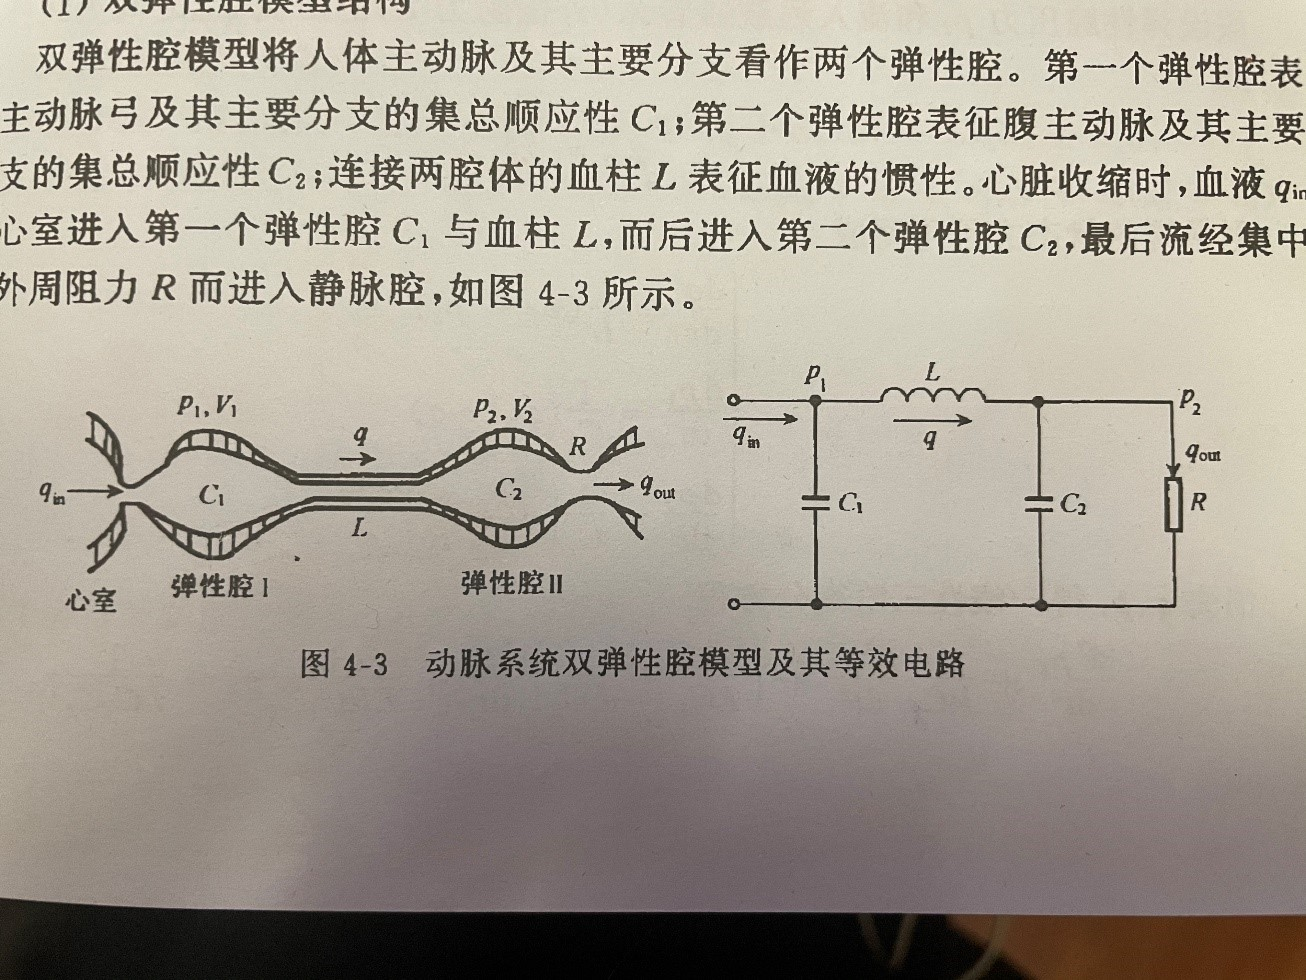
\includegraphics[width=.7\linewidth]{pe/double}
    \caption[动脉系统双弹性腔模型及其等效电路图]{\label{fig:double}动脉系统双弹性腔模型及其等效电路图\cite{PPGYY}}
\end{figure}

对于第一个弹性腔室,血液输入输出关系满足:
\begin{equation}
    \label{equ:QS1}
    q_{in}-q=\frac{\mathrm{d} V_{1}}{\mathrm{d} t}
\end{equation}
对于第二个弹性腔室,血液输入输出关系满足:
\begin{equation}
    \label{equ:QS2}
    q-q_{out}=\frac{\mathrm{d} V_{2}}{\mathrm{d} t}
\end{equation}
设腔室容积$V$与压力$p$之间为线性关系,则有:
\begin{equation}
    \label{equ:QSV1}
    \frac{\mathrm{d} V_{1}}{\mathrm{d} t}
    =\frac{\mathrm{d} V_{1}}{\mathrm{d} p_{1}}\frac{\mathrm{d} p_{1}}{\mathrm{d} t}
    =c_{1}\frac{\mathrm{d} p_{1}}{\mathrm{d} t}
\end{equation}
\begin{equation}
    \label{equ:QSV2}
    \frac{\mathrm{d} V_{2}}{\mathrm{d} t}
    =\frac{\mathrm{d} V_{2}}{\mathrm{d} p_{2}}\frac{\mathrm{d} p_{2}}{\mathrm{d} t}
    =c_{2}\frac{\mathrm{d} p_{2}}{\mathrm{d} t}
\end{equation}
不失一般性,设腔体1、2之间的血液流淌在长度为$l$,截面积为$A$的刚性管道之中。依据动量守恒,则有:
\begin{equation}
    \label{equ:QM}
    \frac{\mathrm{d}}{\mathrm{d} t}\left ( \rho Al\frac{q}{A} \right )=p_{1}A-p_{2}A
\end{equation}
其中,$\rho$为血液密度,$q$为容积流量,$q/A$为血流速度。
\autoref{equ:QM}可进一步简化为
\begin{equation}
    \left \{
    \begin{aligned}
        L\frac{\mathrm{d} q}{\mathrm{d} t} &= p_{1}-p_{2} \\
        L &=\rho \frac{l}{A} \text{(血流惯性)}
    \end{aligned}
    \right.
\end{equation}
设弹性腔压力$p_{2}$和流入血管床的血流$q_{out}$之间为线性关系,即
\begin{equation}
    \label{equ:pq}
    q_{out}=\frac{p_{2}}{R}
\end{equation}
则系统的状态方程可写成
\begin{equation}
    \left \{
    \begin{aligned}
        \frac{\mathrm{d} q}{\mathrm{d} t} &= \frac{1}{L}(p_{1}-p_{2}) \\
        \frac{\mathrm{d} p_{1}}{\mathrm{d} t} &= \frac{1}{C_{1}}(q_{in}-q) \\
        \frac{\mathrm{d} p_{2}}{\mathrm{d} t} &= \frac{1}{C_{2}}(q-\frac{p_{2}}{R}) \\
    \end{aligned}
    \right.
\end{equation}
进一步化简,消除$q$、$p_{1}$可得到:
\begin{equation}
    \label{equ:diff}
    \frac{\mathrm{d^3} p_{2}}{\mathrm{d} t^3}+\frac{1}{RC_{2}}\frac{\mathrm{d}^2p_{2} }{\mathrm{d} t^2}+
    (\frac{1}{LC_{1}}+\frac{1}{LC_{2}})\frac{\mathrm{d} p_{2}}{\mathrm{d} t}+\frac{1}{LRC_{1}C_{2}}p_{2}
    =\frac{1}{LC_{1}C_{2}}q_{in}
\end{equation}
求解该线性三阶微分方程的特征方程,可得
\begin{equation}
    \label{equ:character}
    S^3+\frac{1}{RC_{2}}S^2+(\frac{1}{LC_{1}}+\frac{1}{LC_{2}})S+\frac{1}{LRC_{1}C_{2}}=0
\end{equation}
该特征方程的解由三个分量组成,即直流分量、非震荡衰减分量和震荡衰减分量三部分,可对PPG的主波、潮波和重搏波等主要特征点进行较好的描绘。

2、微循环容积脉搏血流模型

微循环容积脉搏血流模型是刘静纨等\cite{Liu2001}在双弹性腔模型上修正、补充而来。微循环容积脉搏血流模型着重关注了弹性腔中较为笼统的外周阻力,对其进行了进一步的建模,增加了一个
由参数$R$、$L$、$C$组成的二阶系统,如\autoref{fig:micro}所示。
\begin{figure}[htbp]
    \centering
    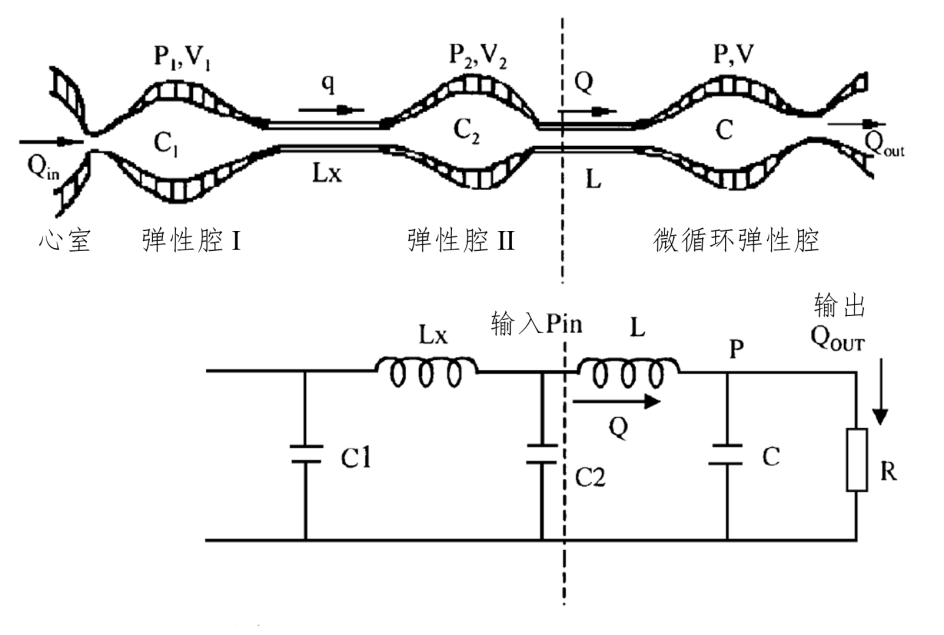
\includegraphics[width=.6\linewidth]{pe/micro}
    \caption[微循环容积脉搏血流模型示意图]{\label{fig:micro}微循环容积脉搏血流模型示意图\cite{PPGYY}}
\end{figure}

根据输入输出关系及该过程中动量守恒,可到微循环弹性腔血流模型的数学表达式为
\begin{equation}
    \label{equ:wxh1}
    \left \{
    \begin{aligned}
        \frac{\mathrm{d} Q}{\mathrm{d} t} &=\frac{P_{in}-P}{L}\\
        \frac{\mathrm{d} P}{\mathrm{d} t} &=\frac{Q-Q_{out}}{C}\\
        Q_{out} &=\frac{P}{R}
    \end{aligned}
    \right.
\end{equation}
消去$P$、$Q$,同样可得一线性三阶微分方程:
\begin{equation}
    \label{equ:wxh2}
    \frac{\mathrm{d^2} Q_{out}}{\mathrm{d} t^2}+\frac{1}{RC}\frac{\mathrm{d} Q_{out}}{\mathrm{d} t}+\frac{1}{LC}Q_{out}=\frac{1}{RLC}P_{in}
\end{equation}
与\autoref{equ:character}类似,这里也可以得到该微分方程的特征方程:
\begin{equation}
    \label{equ:character2}
    S^2+\frac{1}{LC}S+\frac{1}{LC}=0
\end{equation}
易得其传递函数为
\begin{equation}
    \label{equ:hs}
    \begin{aligned}
    G(s) &=\frac{Q_{out}(s)}{P_{in}(s)}=\frac{\frac{1}{RLC}}{S^2+\frac{1}{RC}S+\frac{1}{LC}} \\
    &=\frac{1}{RLC}\frac{1}{2\sqrt{(\frac{1}{2RC})^2-\frac{1}{LC}}}(\frac{1}{S-S_{1}}-\frac{1}{S-S_{2}})
    \end{aligned}
\end{equation}
其中,
\begin{equation}
    \label{equ:ss}
    \left \{
    \begin{aligned}
        S_{1} &= -\frac{1}{2RC}+\sqrt{(\frac{1}{2RC})^2-\frac{1}{LC}}\\
        S_{2} &= -\frac{1}{2RC}-\sqrt{(\frac{1}{2RC})^2-\frac{1}{LC}}\\
    \end{aligned}
    \right.
\end{equation}

二、非生理参数模型

非生理参数模型使用黑箱方法,不追求任何细节,仅通过输入输出信息来研究推导心血管系统模型,具有建立模型过程简单与不破坏系统任何原有结构等优势。

由于PPG信号具有较强的随机性,且其时变特性符合平稳随机信号的定义,可以采用平稳随机信号的线性模型对PPG进行建模分析\cite{Qiu2012,PPGYY,Ma2015}。因此,PPG信号$X(n)$可以看作是某一线性系统在
白噪声$W(n)$的激励下而得到的响应,典型的随机信号参数模型如\autoref{fig:eq}所示。因此,只要确定了白噪声的相关参数,便可以将对PPG的研究转换成对随机信号的线性系统的研究。
\begin{figure}[htbp]
    \centering
    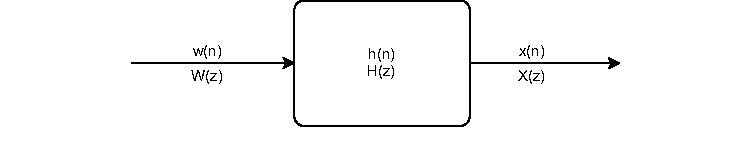
\includegraphics[width=.5\linewidth]{pe/eq}
    \caption{\label{fig:eq}随机信号的参数模型示意图}
\end{figure}

根据系统传递函数形式的不同,可以将平稳随机信号的线性参数模型分为滑动平均(moving average,MA)模型,自回归(autoregressive,AR)模型及自回归滑动平均模型(autoregressive moving average,ARMA)模型等三种。其中,
ARMA模型是AR模型与MA模型的组合,表示脉搏波信号$X(n)$是由自身若干过去值$X(n-k)$与激励时的白噪声$W(n)$及若干白噪声过去值$W(n-k)$线性组合产生的,即:
\begin{equation}
    \label{equ:ARMA}
    X(n)=-\sum_{k=1}^{p}a_{k}X(n-k)+\sum_{k=0}^{q}b_{k}W(n-k)
\end{equation}
对\autoref{equ:ARMA}进行$z$变换,则可得到ARMA模型的传递函数为:
\begin{equation}
    \label{equ:ARMAH}
    H(Z)=\frac{X(Z)}{W(Z)}=\frac{\sum_{k=0}^{q}b_{k}Z^{-k}}{1+\sum_{k=1}^{p}a_{k}Z^{-k}}=\frac{B(Z)}{A(Z)}
\end{equation}
由\autoref{equ:ARMAH}可知,ARMA模型既有零点,也有极点,是零极点模型。一般将ARMA模型记作$ARMA_{(p,q)}$,其中$p$与$q$分别是AR模型与MA模型的阶次。
对\autoref{equ:ARMA}进行傅里叶变换,可进一步得到ARMA模型的功率谱估计为\cite{Qiu2012}:
\begin{equation}
    \label{equ:ARMAP}
    \hat{P}_{ARMA}(e^{j\omega} )=
    \delta _{\omega}^2\left |  \frac{\sum_{k=0}^{p}\hat{b}_{k}e^{-j\omega}}{\sum_{k=0}^{q}\hat{a}_{k}e^{-j\omega}}\right |^2
    =\delta _{\omega}^2\left |  \frac{\hat{B(e^{j\omega} )}}{\hat{A}(e^{j\omega} )}\right |^2
\end{equation}

与上小节中的双弹性腔三阶模型类似,实际证明,当采用ARMA的三阶模型$ARMA_{(3,2)}$来拟合实际PPG波形时,模型输出与实测波形拟合度高、误差小\cite{PPGYY}。在此情形下,PPG波形可由源自\autoref{equ:ARMA}的
\begin{equation}
    \label{equ:ARMA32}
    \begin{aligned}
        X(n)=&-a_{1}X(n-1)-a_{2}X(n-2)-a_{3}X(n-3)\\
        &+b_{0}W(n)+b_{1}X(n-1)+b_{2}W(n-2)
    \end{aligned}
\end{equation}
来表征。模型对应的传递函数为
\begin{equation}
    \label{equ:ARMAH32}
    \begin{aligned}
        H(Z)&=\frac{X(Z)}{W(Z)}=\frac{b_{0}+b_{1}Z^{-1}+b_{2}Z^{-2}}{1+a_{1}Z^{-1}+a_{2}Z^{-2}+a_{3}Z^{-3}}\\
        &=g_{0}+g_{1}Z^{-1}+g_{2}Z^{-2}+...+g_{N-1}Z^{N-1}
    \end{aligned}
\end{equation}
其中,$g_{i}$为PPG实际采样数值,$N$为采样点数。
此时,求解模型则转换成求解\autoref{equ:ARMA32}中相应的$a_{i}$、$b_{i}$系数,使模型拟合曲线与原曲线均方差和最小,即满足:
\begin{equation}
    \label{equ:MeanSum}
    \Delta_{min}=\sum_{i=1}^{N}\left |  (g_i-g'_i)^2\right |
\end{equation}
其中$g'_i$为模型拟合数值。

\subsection{脉搏波的通讯模型}
通信工程中认为,信息是事物运动状态或存在方式的不确定性描述,是通信的内涵;消息是能够被人体感觉器官所感知的物理现象,是信息的外在表现形式;信号则是消息的物理表现形式,是消息的载体\cite{Shannon1948,Liu2019,Zhao2017}。
通讯系统的抽象模型如\autoref{fig:communication}所示。

在\autoref{fig:communication}中,信源是产生消息的源头,是通信的起点。信道是信息的传输媒介,是对实际传输过程的抽象。由于信息的传输过程中会难以避免的引入噪声与干扰,
一般将通讯系统各部分所受到的干扰与噪声折合成信道干扰。为保证传输质量与通讯稳定,编码与解码过程是按照预设的规则对消息符号进行加密和解密的处理过程。
而信宿则是信息传输的目的地,也是接收消息的对象,是本次通信的终点\cite{Zhao2017}。

\begin{figure}[htbp]
    \centering
    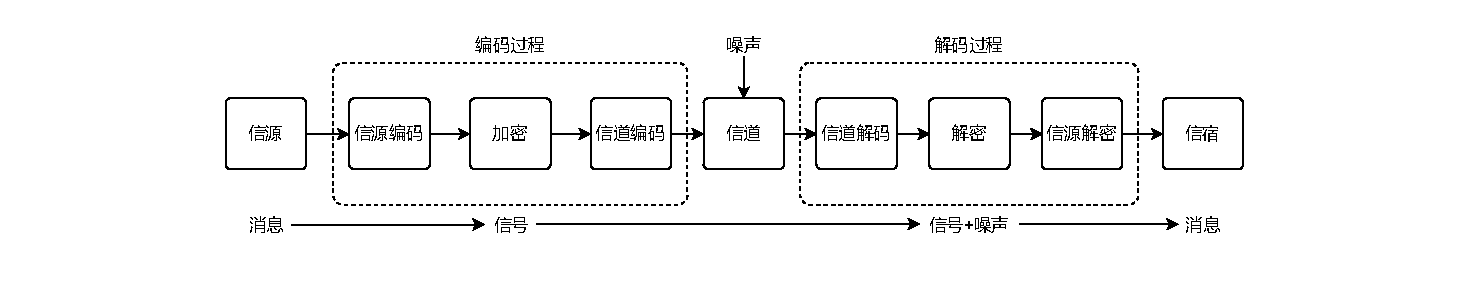
\includegraphics[width=\linewidth]{pe/communication}
    \caption[通讯系统的抽象模型示意图]{\label{fig:communication}通讯系统的抽象模型示意图\cite{Zhao2017,Liu2019}}
\end{figure}

\begin{figure}[htbp]
    \centering
    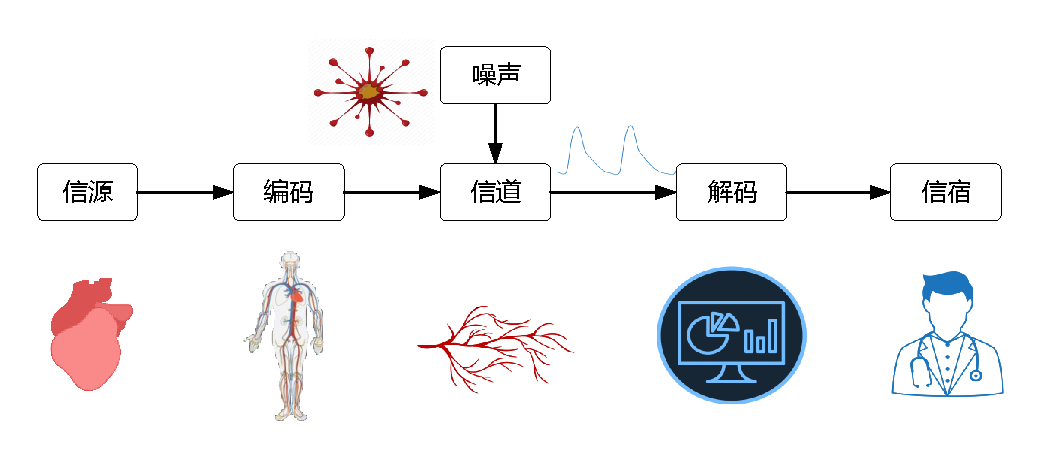
\includegraphics[width=\linewidth]{pe/ppgcommunication}
    \caption{\label{fig:ppgcommunication}人体电生理信号的抽象通讯模型示意图}
\end{figure}

若将人体电生理信号的分析研究问题也抽象成一个通信过程,那么该通讯过程即为人体特定的生理信息从具体器官到临床医生或研究学者之间的信息传输问题,如\autoref{fig:ppgcommunication}所示。
其中,搏动不止的心脏是该系统的信源,人体内各脏器系统、组织等可以看成是一个复杂的黑箱编码系统,人体表面丰富的毛细血管则是
该通讯过程中的信道,由PE等疾病引起的人体毛细血管等系统的生理性变化可以折合成对信道的干扰噪声。而PPG信号可以看成是反映信源——心脏功能与信道——人体血液循环系统的特性的特殊消息载体。
在此基础上,\textbf{PPG的描述过程可视为在编码规则不明确(黑箱模型)的前提下对其携带的生理信息进行译码解码的过程。}

另一方面,在对PPG信号分析时,其输入均是以数值形式的采样值序列。不论是类似“该波形周期较长”、“该波形重搏波、潮波不明显”等自然语言描述,
还是以“下降支时长为0.43s”、“该波形波峰幅值为1351”等绝对量化的数值描述,均是以较少的数值去完成PPG信号的描述与评估过程。因此,\textbf{对PPG信号的数字量化过程也是一个信息压缩过程。}

\section{小结}
本章内容对PE的生理学特性与其可引起的病生理变化进行了介绍。介绍了PPG信号的产生原理与采集原理,从人体电生理信号的共性特征与PPG信号的个性特征对PPG的特征进行了说明。
也对PPG分析过程中常使用的生理参数模型与非生理参数模型进行了说明。
最后,按方法论的观点从通讯原理的角度,概括PPG的通讯模型。本章的研究为后续研究提供了理论基础。